\documentclass[12pt,letterpaper]{article}
\usepackage{graphicx,textcomp}
\usepackage{natbib}
\usepackage{setspace}
\usepackage{fullpage}
\usepackage{color}
\usepackage[reqno]{amsmath}
\usepackage{amsthm}
\usepackage{fancyvrb}
\usepackage{amssymb,enumerate}
\usepackage[all]{xy}
\usepackage{endnotes}
\usepackage{lscape}
\newtheorem{com}{Comment}
\usepackage{float}
\usepackage{hyperref}
\newtheorem{lem} {Lemma}
\newtheorem{prop}{Proposition}
\newtheorem{thm}{Theorem}
\newtheorem{defn}{Definition}
\newtheorem{cor}{Corollary}
\newtheorem{obs}{Observation}
\usepackage[compact]{titlesec}
\usepackage{dcolumn}
\usepackage{tikz}
\usetikzlibrary{arrows}
\usepackage{multirow}
\usepackage{xcolor}
\newcolumntype{.}{D{.}{.}{-1}}
\newcolumntype{d}[1]{D{.}{.}{#1}}
\definecolor{light-gray}{gray}{0.65}
\usepackage{url}
\usepackage{listings}
\usepackage{color}

\definecolor{codegreen}{rgb}{0,0.6,0}
\definecolor{codegray}{rgb}{0.5,0.5,0.5}
\definecolor{codepurple}{rgb}{0.58,0,0.82}
\definecolor{backcolour}{rgb}{0.95,0.95,0.92}

\lstdefinestyle{mystyle}{
	backgroundcolor=\color{backcolour},   
	commentstyle=\color{codegreen},
	keywordstyle=\color{magenta},
	numberstyle=\tiny\color{codegray},
	stringstyle=\color{codepurple},
	basicstyle=\footnotesize,
	breakatwhitespace=false,         
	breaklines=true,                 
	captionpos=b,                    
	keepspaces=true,                 
	numbers=left,                    
	numbersep=5pt,                  
	showspaces=false,                
	showstringspaces=false,
	showtabs=false,                  
	tabsize=2
}
\lstset{style=mystyle}
\newcommand{\Sref}[1]{Section~\ref{#1}}
\newtheorem{hyp}{Hypothesis}

\title{Problem Set 7}
\date{Due: May 1, 2020}
\author{QTM 200: Applied Regression Analysis}

\begin{document}
	\maketitle
	
	\section*{Instructions}
	\begin{itemize}
		\item Please show your work! You may lose points by simply writing in the answer. If the problem requires you to execute commands in \texttt{R}, please include the code you used to get your answers. Please also include the \texttt{.R} file that contains your code. If you are not sure if work needs to be shown for a particular problem, please ask.
		\item Your homework should be submitted electronically on the course GitHub page in \texttt{.pdf} form.
		\item This problem set is due before midnight on Friday, May 1, 2020. No late assignments will be accepted.
		\item Total available points for this homework is 100.
	\end{itemize}
	
	\vspace{.5cm}

\section*{Question 1 (50 points): Political Science}	
\noindent Consider the data set \texttt{MexicoMuniData.csv}, which includes municipal-level information from Mexico. The outcome of interest is the number of times the winning PAN presidential candidate in 2006 (\texttt{PAN.visits.06}) visited a district leading up to the 2009 federal elections, which is a count. Our main predictor of interest is whether the district was highly contested, or whether it was not (the PAN or their opponents have electoral security) in the previous federal elections during 2000 (\texttt{competitive.district}), which is binary (1=close/swing district, 0="safe seat"). We also include \texttt{marginality.06} (a measure of poverty) and \texttt{PAN.governor.06} (a dummy for whether the state has a PAN-affiliated governor) as additional control variables. 

\begin{enumerate}
	\item [(a)]
	Run a Poisson regression because the outcome is a count variable. Is there evidence that PAN presidential candidates visit swing districts more? Provide a test statistic and p-value. 
	
	\lstinputlisting[language=R, firstline=48, lastline=50]{PS07_answers.R}
	
	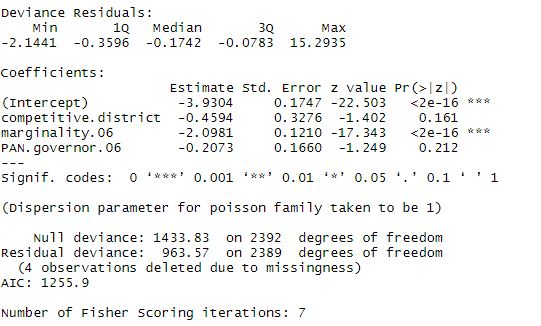
\includegraphics[scale=.75]{summary table 1.jpg}

	\newpage 
	
	\item [(b)]
	Interpret the \texttt{marginality.06} and \texttt{PAN.governor.06} coefficients. 
	
	\lstinputlisting[language=R, firstline=54, lastline=54]{PS07_answers.R}
	
	\item [(c)]
	Provide the estimated mean number of visits from the winning PAN presidential candidate for a hypothetical district that was competitive (\texttt{competitive.district}=1), had an average poverty level (\texttt{marginality.06} = 0), and a PAN governor (\texttt{PAN.governor.06}=1). 
	
	\lstinputlisting[language=R, firstline=58, lastline=58]{PS07_answers.R}
	
\end{enumerate}
	

\section*{Question 2 (50 points): Biology}
\noindent We'll be using data from a longitudinal sleep study of under 20 undergraduate students ($n$=18), which took place over the course of 10 days to see if sleep deprivation has any effect on participants' reaction time. Load the data through the \texttt{lmer} package.

\begin{enumerate}
	\item
	Create a "pooled" linear model where you regress \texttt{Days} on the outcome \texttt{Reaction}. Make sure to run regression diagnostics to check if the variance around the regression line is equal for every year. 
	
	\lstinputlisting[language=R, firstline=66, lastline=67]{PS07_answers.R} 
	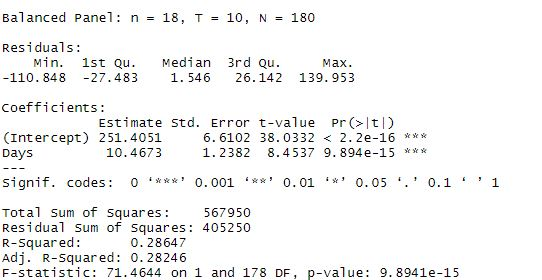
\includegraphics[scale=.75]{summary table 2.jpg}
	
	\item Fit an "un-pooled" regression model with varying intercepts for patient (include an additive factor for patient) and save the fitted values. 
	
	\lstinputlisting[language=R, firstline=70, lastline=71]{PS07_answers.R} 
	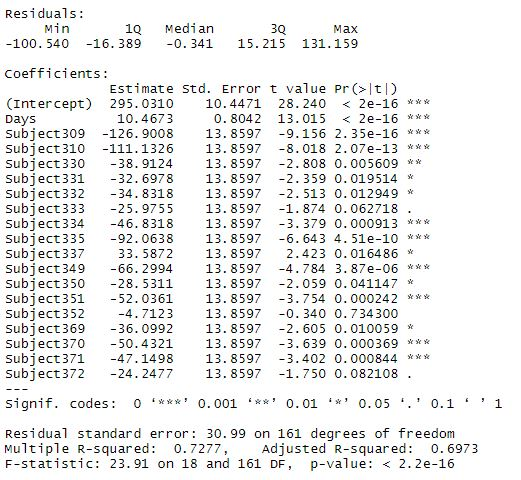
\includegraphics[scale=.75]{summary table 3.jpg}
	
	\item Fit a "un-pooled" regression model with varying slopes of time (days) for patients (include only the interaction \texttt{Days:Subject}) and save the fitted values. 
	
	\lstinputlisting[language=R, firstline=74, lastline=75]{PS07_answers.R} 
	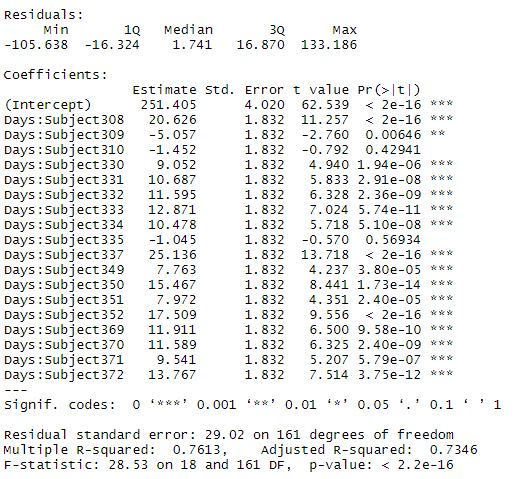
\includegraphics[scale=.75]{summary table 4.jpg}
	
	\item Fit an "un-pooled" regression model with varying intercepts for patients with varying slopes of time (days) by patient (include the interaction and constituent terms of \texttt{Days} and \texttt{Subject}, \texttt{Days + Subject + Days:Subject}) and save the fitted values. 
	
	\lstinputlisting[language=R, firstline=78, lastline=79]{PS07_answers.R} 
	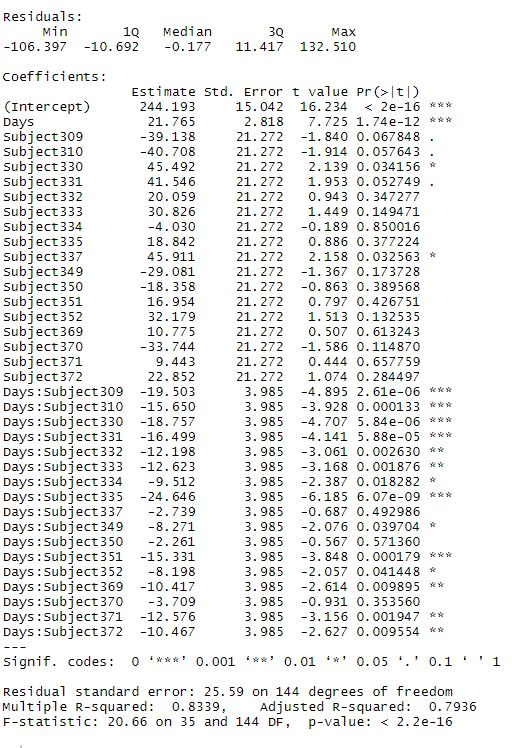
\includegraphics[scale=.75]{summary table 5.jpg}
	
	\item Fit a "semi-pooled" multi-level model with varying-intercept for subject and varying-slope of day by subject. Is it worthwhile for us to run a multi-level model with varying effects of time by subject? Why? Compare your model from part 5 to the other completely "pooled" or "un-pooled models". 
	
	\lstinputlisting[language=R, firstline=82, lastline=84]{PS07_answers.R} 
	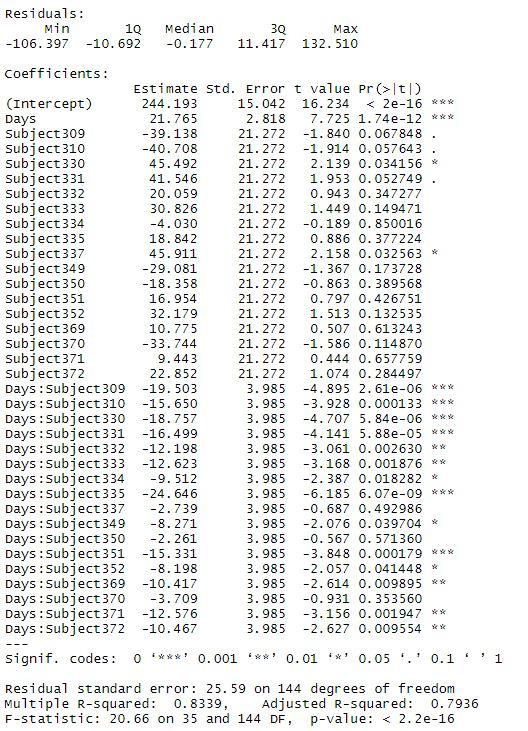
\includegraphics[scale=.75]{summary table 6.jpg}

\end{enumerate}

\end{document}
=======
\documentclass[12pt,letterpaper]{article}
\usepackage{graphicx,textcomp}
\usepackage{natbib}
\usepackage{setspace}
\usepackage{fullpage}
\usepackage{color}
\usepackage[reqno]{amsmath}
\usepackage{amsthm}
\usepackage{fancyvrb}
\usepackage{amssymb,enumerate}
\usepackage[all]{xy}
\usepackage{endnotes}
\usepackage{lscape}
\newtheorem{com}{Comment}
\usepackage{float}
\usepackage{hyperref}
\newtheorem{lem} {Lemma}
\newtheorem{prop}{Proposition}
\newtheorem{thm}{Theorem}
\newtheorem{defn}{Definition}
\newtheorem{cor}{Corollary}
\newtheorem{obs}{Observation}
\usepackage[compact]{titlesec}
\usepackage{dcolumn}
\usepackage{tikz}
\usetikzlibrary{arrows}
\usepackage{multirow}
\usepackage{xcolor}
\newcolumntype{.}{D{.}{.}{-1}}
\newcolumntype{d}[1]{D{.}{.}{#1}}
\definecolor{light-gray}{gray}{0.65}
\usepackage{url}
\usepackage{listings}
\usepackage{color}

\definecolor{codegreen}{rgb}{0,0.6,0}
\definecolor{codegray}{rgb}{0.5,0.5,0.5}
\definecolor{codepurple}{rgb}{0.58,0,0.82}
\definecolor{backcolour}{rgb}{0.95,0.95,0.92}

\lstdefinestyle{mystyle}{
	backgroundcolor=\color{backcolour},   
	commentstyle=\color{codegreen},
	keywordstyle=\color{magenta},
	numberstyle=\tiny\color{codegray},
	stringstyle=\color{codepurple},
	basicstyle=\footnotesize,
	breakatwhitespace=false,         
	breaklines=true,                 
	captionpos=b,                    
	keepspaces=true,                 
	numbers=left,                    
	numbersep=5pt,                  
	showspaces=false,                
	showstringspaces=false,
	showtabs=false,                  
	tabsize=2
}
\lstset{style=mystyle}
\newcommand{\Sref}[1]{Section~\ref{#1}}
\newtheorem{hyp}{Hypothesis}

\title{Problem Set 7}
\date{Due: May 6, 2020}
\author{QTM 200: Applied Regression Analysis}

\begin{document}
	\maketitle
	
	\section*{Instructions}
	\begin{itemize}
		\item Please show your work! You may lose points by simply writing in the answer. If the problem requires you to execute commands in \texttt{R}, please include the code you used to get your answers. Please also include the \texttt{.R} file that contains your code. If you are not sure if work needs to be shown for a particular problem, please ask.
		\item Your homework should be submitted electronically on the course GitHub page in \texttt{.pdf} form.
		\item This problem set is due before midnight on Wednesday, May 6, 2020. No late assignments will be accepted.
		\item Total available points for this homework is 100.
	\end{itemize}
	
	\vspace{.5cm}

\section*{Question 1 (50 points): Political Science}	
\noindent Consider the data set \texttt{MexicoMuniData.csv}, which includes municipal-level information from Mexico. The outcome of interest is the number of times the winning PAN presidential candidate in 2006 (\texttt{PAN.visits.06}) visited a district leading up to the 2009 federal elections, which is a count. Our main predictor of interest is whether the district was highly contested, or whether it was not (the PAN or their opponents have electoral security) in the previous federal elections during 2000 (\texttt{competitive.district}), which is binary (1=close/swing district, 0="safe seat"). We also include \texttt{marginality.06} (a measure of poverty) and \texttt{PAN.governor.06} (a dummy for whether the state has a PAN-affiliated governor) as additional control variables. 

\begin{enumerate}
	\item [(a)]
	Run a Poisson regression because the outcome is a count variable. Is there evidence that PAN presidential candidates visit swing districts more? Provide a test statistic and p-value.
	\newpage
	\item [(b)]
	Interpret the \texttt{marginality.06} and \texttt{PAN.governor.06} coefficients.
	
	\item [(c)]
	Provide the estimated mean number of visits from the winning PAN presidential candidate for a hypothetical district that was competitive (\texttt{competitive.district}=1), had an average poverty level (\texttt{marginality.06} = 0), and a PAN governor (\texttt{PAN.governor.06}=1).
	
\end{enumerate}
	

\section*{Question 2 (50 points): Biology}
\noindent We'll be using data from a longitudinal sleep study of under 20 undergraduate students ($n$=18), which took place over the course of 10 days to see if sleep deprivation has any effect on participants' reaction time. Load the data through the \texttt{lmer} package.

\begin{enumerate}
	\item
	Create a "pooled" linear model where you regress \texttt{Days} on the outcome \texttt{Reaction}. Make sure to run regression diagnostics to check if the variance around the regression line is equal for every year.
	
	\item Fit an "un-pooled" regression model with varying intercepts for patient (include an additive factor for patient) and save the fitted values.
	
	\item Fit a "un-pooled" regression model with varying slopes of time (days) for patients (include only the interaction \texttt{Days:Subject}) and save the fitted values.
	
	\item Fit an "un-pooled" regression model with varying intercepts for patients with varying slopes of time (days) by patient (include the interaction and constituent terms of \texttt{Days} and \texttt{Subject}, \texttt{Days + Subject + Days:Subject}) and save the fitted values.
	
	\item Fit a "semi-pooled" multi-level model with varying-intercept for subject and varying-slope of day by subject. Is it worthwhile for us to run a multi-level model with varying effects of time by subject? Why? Compare your model from part 5 to the other completely "pooled" or "un-pooled models".

\end{enumerate}

\end{document}
>>>>>>> upstream/master
